%-------------------------------------------------------------------------------
\section{Event reconstruction and selections\label{sec:Selections}}

	%--------------------------------------------------------------------------------
	\subsection{Event reconstruction\label{subsec:EventReconstruction}}
The muons, electrons, jets and missing transverse energy (\MET) reconstruction and criteria are described in
in details in~\cite{AN-2012-194}. The following criteria are only a brief summary:
\begin{itemize}
\item {\bf Muons:} {\it GlobalMuon} 
                   (with $\chi^2/ndof < 10$, at least one good muon hit and at least two muon segments in different muon stations)  
                   or {\it TrackerMuon}  (provided it satisfies the "Tracker Muon Last Station Tight" selection). Several cut-based identification 
                   criteria are applied as well as the particle flow (PF) Isolation. In 2012, the PF Isolation is replaced
                   by an MVA algorithm.
\item {\bf Electrons:} {\it GSF Electons}. A MVA identification criteria is applied  as well as an MVA algorithm.
\item {\bf Jets:}  {\it Anti-$k_T$ PF jets} (with R=0.5 and applying L1, L2 and L3 jet energy corrections, including Pile-Up jet corrections from Fastjet method). Only jets and $|\eta|<4.7$ are considered. A specific Pile-Up MVA-based rejection algorithm is applied.   
\item {\bf \MET:}  The \MET is reconstructed the {\it PF Algorithm} or considering {\it only tracks} originating from the same vertex as 
                   the two leptons. In addition, the minimum of the projections of these two \MET to the closest lepton direction if they are in the same hemisphere, otherwise of their original values, is used in the analysis.  
\end{itemize}

	%--------------------------------------------------------------------------------
	\subsection{Event selection\label{subsec:EventSelection}}
Unlike the main \hwwllnn analysis, this analysis is inclusive in number of jets, so we do not have to define different jet multiplicity categories.
The event selection consist of several steps. The first step is to select \WW -like events applying a selection that is heavily based on the main analysis selection except for few different cuts explained below.
The \WW -like event preselection consists of the following set of cuts:
\begin{enumerate}
\item {\bf Lepton preselection}:
  \begin{itemize}
  \item at least two opposite-sign and opposite-flavour ($e\mu$) leptons reconstructed in the event;
  \item $|\eta|<2.5$ for electrons and $|\eta|<2.4$ for muons;
  \item $\pt>20~\GeV$ for the leading lepton. For the trailing lepton, the transverse momentum is required to be larger than 10~\GeV.
  \end{itemize}
\item {\bf Extra lepton veto}: the event is required to have two and only two opposite-sign leptons passing the lepton selection.
\item {\bf \MET preselection}: particle flow \MET is required to be greater than $20$\GeV.
\item {\bf Di-lepton mass cut}: $\mll > 12$\GeV in order to reject low mass resonances and QCD backgrounds.
\item {\bf Di-lepton $p_T$ cut}: $\ptll > 30$\GeV.
\item {\bf projected \MET selection}: minimum projected \MET required to be larger than 20~\GeV.
\item {\bf Transverse mass}: $m_T^H>60$\GeV to reject Drell-Yan to $\tau\tau$ events. 
\end{enumerate}
In addition to the \WW-like preselection other cuts are applied in order to reduce the top background (\ttbar ans single-top), which is one of the main backgrounds in this final state. We operate two different selections depending on the number of jets with $p_T > 30$~\GeV in the event. This is done to suppress the top background both in the low $p_T^H$ region, where 0-jets events have the biggest contribution, and for higher values where also larger jet multiplicity events are important.
The selection for 0-jets events relies on a soft muon veto, which rejects events with non-isolated soft muons (likely belonging to b-jets), and on a soft jets (with $p_T < 30$~\GeV) anti b-tagging requirement.
The latter requirement exploits the Track Counting High Efficiency tagger (TCHE) to reject soft jets that are likely to come from b quarks hadronization.
These are exactly the same requirements applied in the 0-jets bin of the main analysis.

For events with a jet multiplicity greater or equal than one, we apply a different selection with respect to the main analysis. In this case we exploit the good b-tagging performances of the \textit{JetBProbability} tagger to reject all the jets with $\pt > 30$~\GeV that are likely to come from a b quark. This jet veto relies on a cut on the \textit{JetBProbability} tagger discriminant as has been also done in the VH (\hwwllnn) analysis \cite{CMS_PAS_HIG_13-017}. Any jet with a discriminant value below $1.4$ is identified as a non b-jet. The analysis selection requires no b-tagged jets with $\pt > 30$~\GeV.

\begin{figure}[b]
\centering
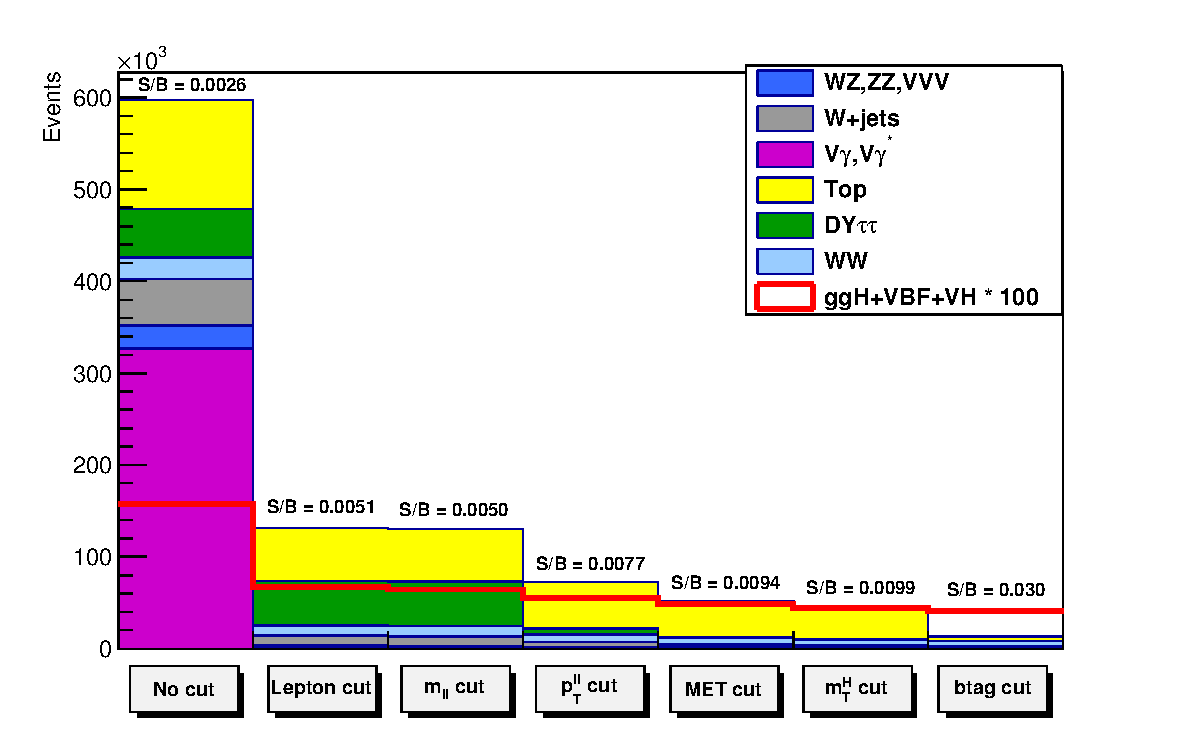
\includegraphics[width=0.8\textwidth]{images/cutflow2.pdf}
\caption{Effect of single selections on MC samples. The signal (red line) is multiplied by 100 and superimposed on stacked backgrounds. In each bin, corresponding to a different selection, is reported the expected number of events in MC at a luminosity of $19.46~\mathrm{fb}^{-1}$.\label{fig:cutflow}}
\end{figure}

A  cut-flow plot is reported in figure \ref{fig:cutflow} showing the effect of each selection on top of Monte Carlo samples. In the first bin, labelled as \textit{No cut}, no selection has been applied and the bin content correspond to the total expected number of events with a luminosity of $19.46~\mathrm{fb}^{-1}$. All the events in this bin have at least two leptons with a loose transverse momentum cut of $8$\GeV. In the following bin the lepton cuts are applied, including the requirement to have two opposite-sign and opposite-flavour leptons and the extra lepton veto. Then are progressively reported all the other selections, showing the effect of each cut on backgrounds and signal. For each selection is also reported the expected signal over background ratio which after the full selection reach a maximum value around $3\%$.

\begin{figure}[t]
\centering
\subfigure[]{
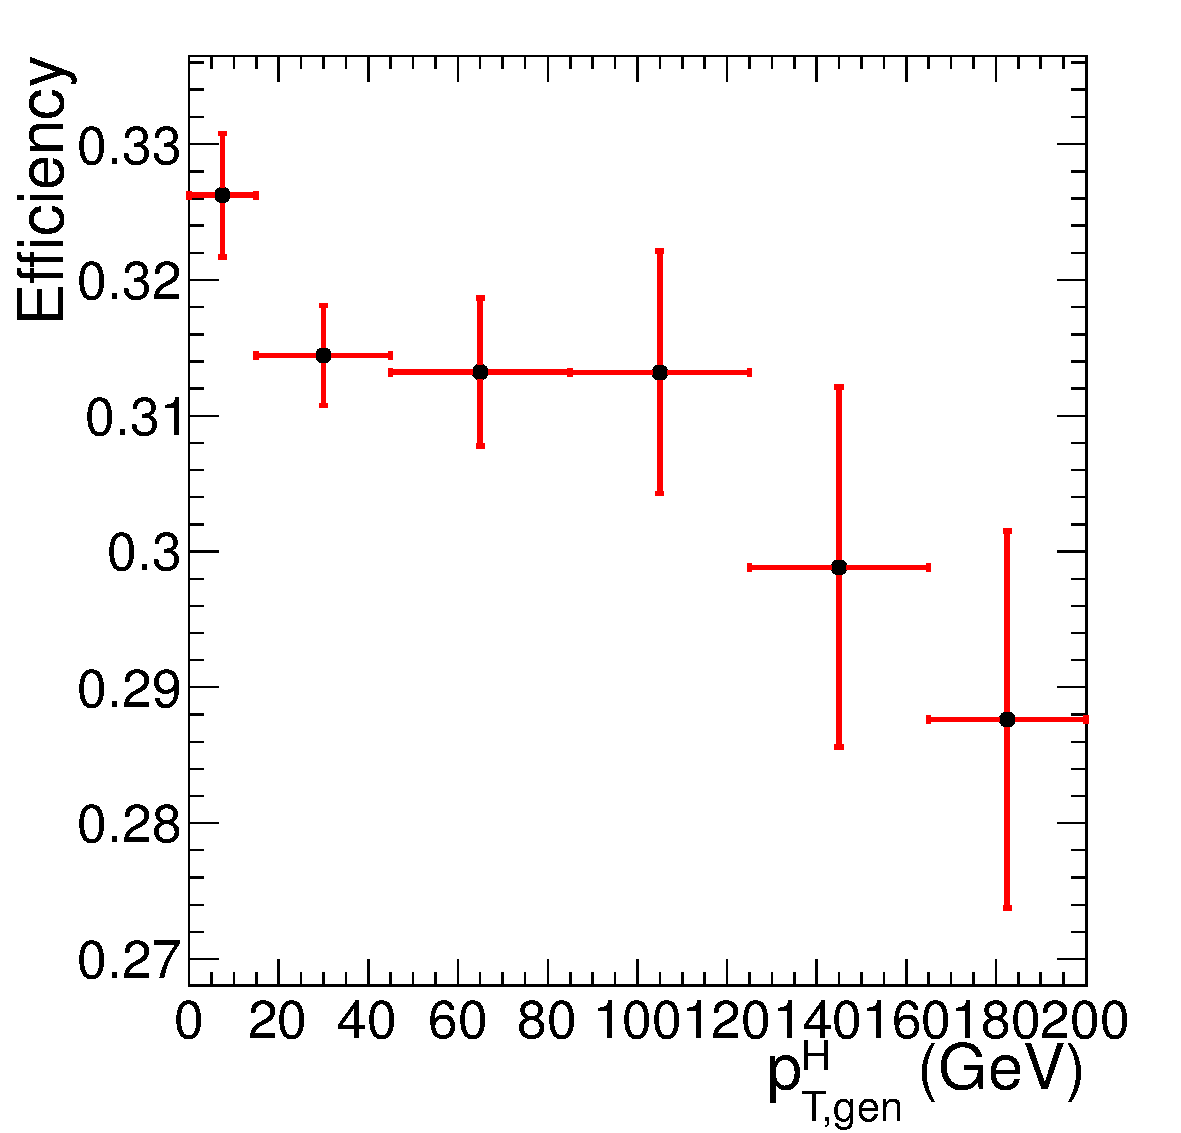
\includegraphics[width=0.4\textwidth]{images/eff_pth.pdf}
}
\subfigure[]{
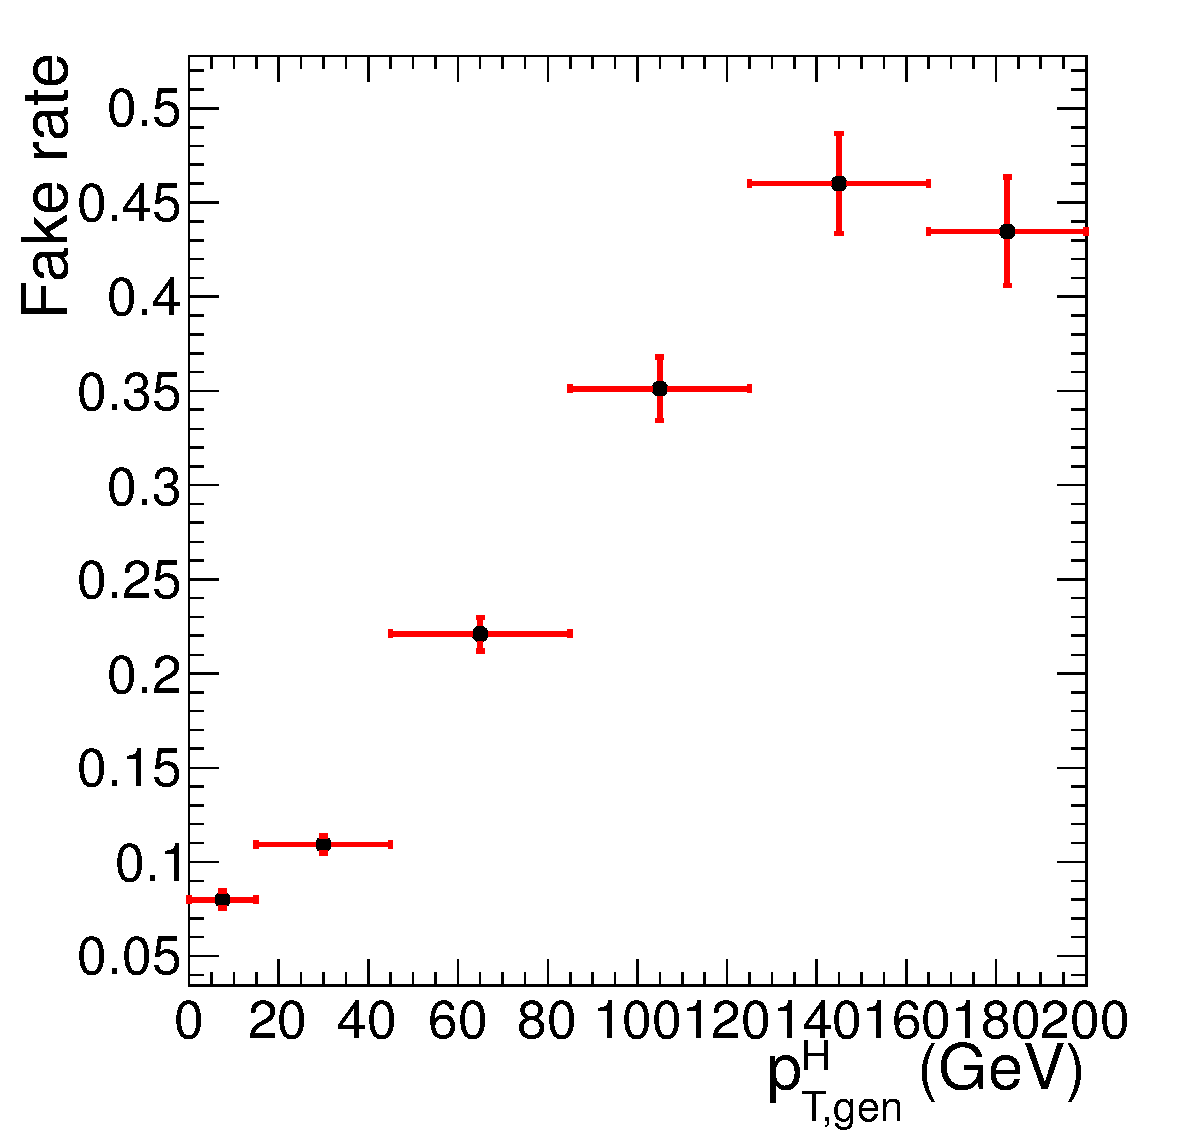
\includegraphics[width=0.4\textwidth]{images/fake_pth.pdf}
}
\caption{Efficiency of the full selection (a) and fake rate (b) as a function of $p_T^H$.\label{fig:sel_eff}}
\end{figure}

The selection efficiency is shown in Fig.~\ref{fig:sel_eff} (a). The efficiency denominator is the number of events that pass the acceptance, while the numerator is the number of events that pass both the selection and the acceptance, in each \pth bin. The fake rate, defined by the ratio of signal events that pass the selection but are not within the acceptance, divided by the total number of events passing both the selection and the acceptance is shown in Fig.~\ref{fig:sel_eff} (b). For both the selection efficiency and the fake rate the signal samples included correspond to the ggH, VBF and VH production mechanisms.
The overall efficiency and fake rate are: $\epsilon=0.362\pm{0.005}$ and $fake~rate=0.126\pm0.004$, where the errors are only statistical.

If a $4\pi$ acceptance is defined, requiring just that the Higgs decays to WW and then to $2\ell2\nu$, the efficiency is $\epsilon=0.03960\pm{0.00033}$. 

